
%(BEGIN_QUESTION)
% Copyright 2012, Tony R. Kuphaldt, released under the Creative Commons Attribution License (v 1.0)
% This means you may do almost anything with this work of mine, so long as you give me proper credit

Rosemount 3244MV FOUNDATION Fieldbus temperaturtransmitter kan ta imot signaler fra termoelementer, RTD-er og generelle millivoltkilder (fra -10 mV til +100 mV). Muligheten til å skalere et millivoltsignal digitalt til ønsket måleområde er svært nyttig. Se denne anvendelsen der vi bruker en Rosemount 3244MV-transmitter til å konvertere signalet fra en turtallsgenerator til hastighetsindikasjon for en motor (RPM):

$$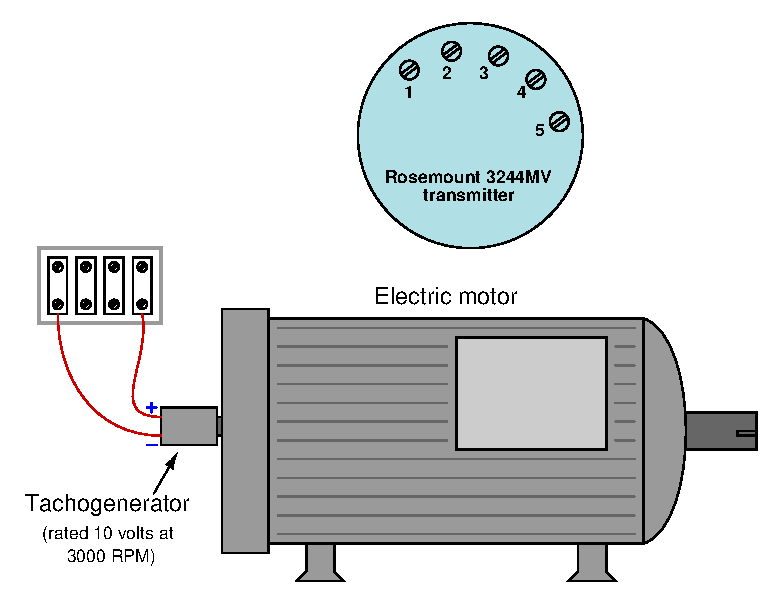
\includegraphics[width=15.5cm]{i01219x01.eps}$$

Turtallsgeneratoren er i praksis en liten permanentmagnetisk DC-generator med utgangsspenning proporsjonal med akselhastigheten (denne er spesifisert til 10 V ved 3000 RPM).

\vskip 10pt

Tegn en krets som kobler turtallsgeneratoren til 3244MV-transmitteren, slik at transmitteren aldri utsettes for mer enn 100 mV signal. Bestem også riktige konfigurasjonsparametere i instrumentets Analog Input (AI)-blokk slik at utgangen skaleres til 0-2500 RPM:

% No blank lines allowed between lines of an \halign structure!
% I use comments (%) instead, so som TeX doesn't choke.

$$\vbox{\offinterlineskip
\halign{\strut
\vrule \quad\hfil # \ \hfil & 
\vrule \quad\hfil # \ \hfil \vrule \cr
\noalign{\hrule}
%
% First row
{\tt L\_Type} & \hskip 50pt \cr
%
\noalign{\hrule}
%
% Another row
{\tt XD\_Scale} & \hskip 50pt \cr
%
\noalign{\hrule}
%
% Another row
{\tt OUT\_Scale} & \hskip 50pt \cr
%
\noalign{\hrule}
} % End of \halign 
}$$ % End of \vbox

\vfil 

\underbar{file i01219}
\eject
%(END_QUESTION)





%(BEGIN_ANSWER)

Dette er en vurderingsoppgave -- ingen svar eller hint er gitt!

%(END_ANSWER)





%(BEGIN_NOTES)

Dette er én mulig løsning:

$$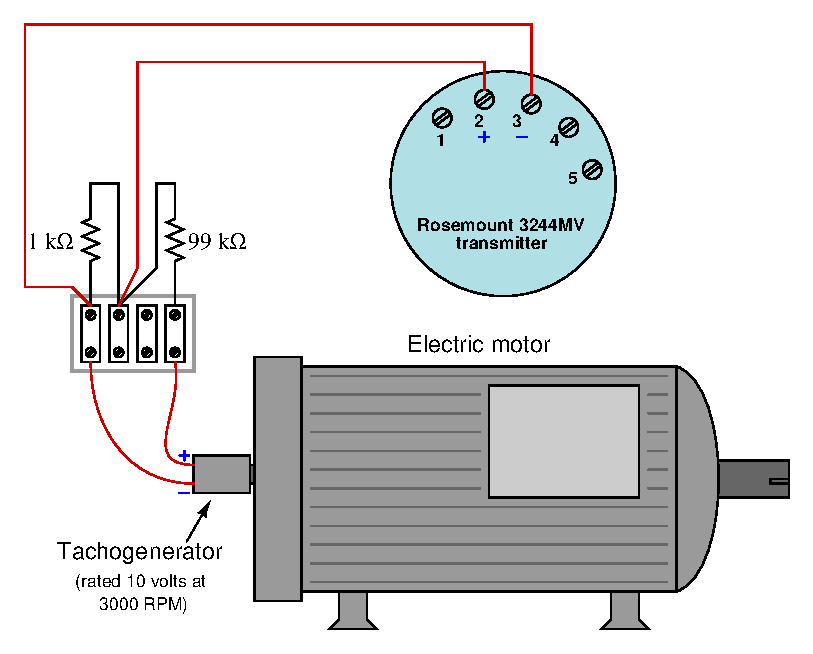
\includegraphics[width=15.5cm]{i01219x02.eps}$$

% No blank lines allowed between lines of an \halign structure!
% I use comments (%) instead, so som TeX doesn't choke.

$$\vbox{\offinterlineskip
\halign{\strut
\vrule \quad\hfil # \ \hfil & 
\vrule \quad\hfil # \ \hfil \vrule \cr
\noalign{\hrule}
%
% First row
{\tt L\_Type} & Indirect \cr
%
\noalign{\hrule}
%
% Another row
{\tt XD\_Scale} & 0 to 83.33 mV \cr
%
\noalign{\hrule}
%
% Another row
{\tt OUT\_Scale} & 0 to 2500 RPM \cr
%
\noalign{\hrule}
} % End of \halign 
}$$ % End of \vbox

\vskip 10pt

Merk at parameteren {\tt OUT\_Scale} er overflødig i denne applikasjonen. Så lenge {\tt L\_Type} er satt til ``Direct'', rapporterer transmitteren det sensoren måler, uavhengig av {\tt OUT\_Scale}-parameterne.

%INDEX% Fieldbus, instrumentområde: innstilling av XD_Scale- og OUT_Scale-parametere

%(END_NOTES)

